
\subsection{CRONOGRAMA DE ACTIVIDADES}

	Las actividades a realizar son las siguientes: 


\begin{enumerate}
	%************** primer objetivo *****************************
	\item Elegir y justificar el uso del lenguaje para el análisis y modelado estadístico.
	\item Elegir y justificar el uso del lenguaje para el análisis en frecuencia.
	\item Elegir y justificar el uso del lenguaje para el manejo y control de la información.
	\item Elegir y justificar el uso del lenguaje para la base de datos.
	\item Elegir y justificar el uso del lenguaje para el muestreo de la información.
	%************** segundo objetivo *****************************
	\item Estudiar la BBDD para obtener un modelo del comportamiento de la vibración en motores eléctricos.
	\item Programar el modelo y su interacción con el servidor.
	%************** tercer objetivo *****************************
	\item Definir y programar el modelo de la base de datos.
	\item Utilizar el programa del modelo estadístico anteriormente generado para llenar la BBDD
	%************** cuarto objetivo *****************************
	\item Crear el programa para dada la entrada de un array de datos(vibración discretizada), obtener la salida del estudio en frecuencia.
	\item Hacer un script con el punto anterior para permitir el llamado desde el servidor. 
	%************** quinto objetivo *****************************
	\item Programar los serializadores para llevar la información de la BBDD al nivel visual solicitado.
	\item Crear la pagina para la vista general.
	\item Crear la pagina para la vista especifica.
	\item Crear la pagina para la vista exhaustiva.
	%************** sexto objetivo *****************************
	\item Elaboración de la pagina web con los objetivos 12 al 15.
	%************** septimo objetivo *****************************
	\item Comprobar los resultados.
\end{enumerate}


	y el cronograma queda de la forma:\\

	\begin{figure}[htb]
		\centering
		\caption{Cronograma de actividades.}
		\label{cronograma}
		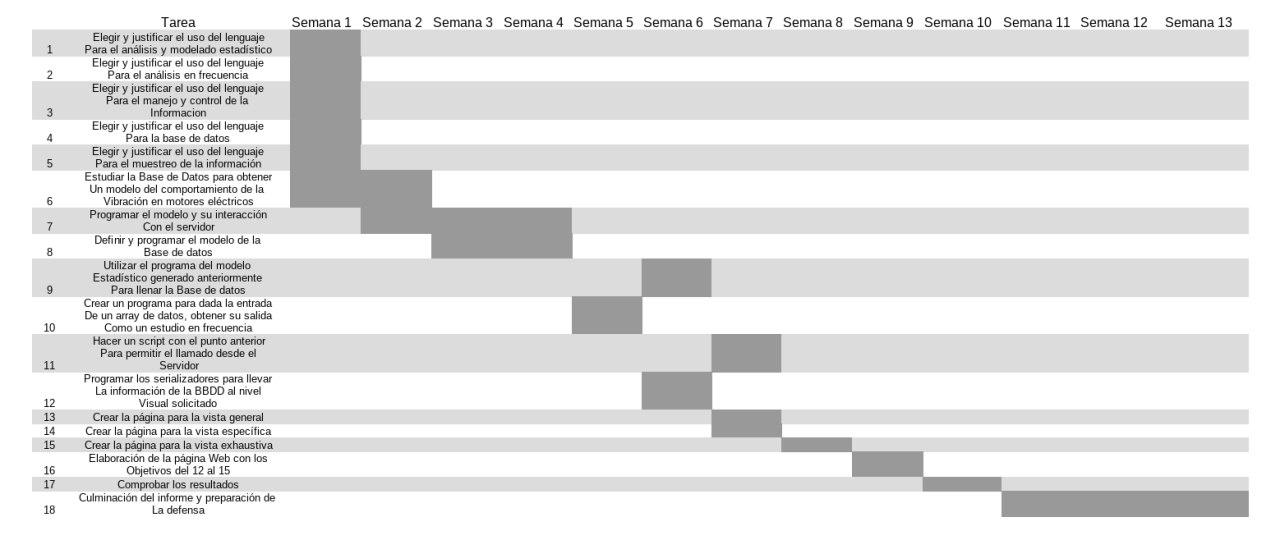
\includegraphics[width=17cm, height=20cm]{diagrama_grant.jpg}
	\end{figure}
